\documentclass{article}
\usepackage[final]{pdfpages}
\title{Riunione 1}
\date{2019-30-11}
\author{Mario Turco}

\begin{document}

\maketitle
\pagenumbering{gobble}
\newpage
\pagenumbering{arabic}
\section{Partecipanti}
\begin{enumerate}
    \item Mario Turco
    \item Francesco Longobardi  
    \item Giuseppe Rauso
\end{enumerate}
\section{Lista di cose da chiedere al Customer}
\begin{enumerate}
    \item Recensione e commento sono entrambi parte dello stesso ogetto? Ovvero, descrizione testauale e valutazione in stelle rappresentano la recensione oppure sono due(stelle, descrizione) oggetti diveri?
    \item È possibile fare una recensione con solo il rating?(Stelle)
    \item È possibile fare una recensione senza rating ma solo testuale?
    \item Utenti e recensori sono la stessa cosa?
    \item L'utente registrato (il recensore) può cambiare altre informazioni del suo profilo oltre al nome utente? Ad esempio cambiando l'email, la password,etc...
    \item Il recensore sceglie se usare il suo vero nome o un nick name. Quest'azione viene fatta al tempo della registrazione può essere cambiata tramite la gestione del profilo oppure va scelta ad ogni inserimento di una nuova recensione?
    \item Cosa significa gestione dei visitatori?
\end{enumerate}
\newpage
\section{Argomenti}
Prima discussione su come iniziare il progetto.
Dobbiamo definire i requisiti funzionali, non funzionali e di dominio (eventuali), definire gli attori e definire i casi d'uso.
Sul forum non c'è materiale rilevante che sia d'aiuto.

\section{Definizione degli attori}
  \paragraph{Lista di attori}
  \begin{enumerate}
      \item Amministratore
      \item Utente Registrato (cliente)
      \item Utente non Registrato (visitatore)
  \end{enumerate}
  \paragraph{Alcune considerazioni}
  A quanto pare la traccia fa una distinzione tra utenti non registrati , chiamati visitatori, ed utente registrati
  che, ad esempio possono lasciare recensioni a differenza dei visitatori.
  Per quanto riguarda gli amministratori, lato "Back Office", potrebbero ulteriormente dividersi in moderatori 
  delle recensioni che sono un sottoinsieme degli amministratori(i quali hanno tutte le funzioni dei moderatori)
 più qualcoshe altra funzione. Ma probabilmente non è una divisiore utile, ne discuteremo più avanti.

 \section{Lista di funzinalità per ogni attore}
 \subsection{Amministratore}
 \begin{enumerate}
    \item Rimuove una recensione
    \item Accettare una recensione
    \item Ricerca strutture già caricate
    \item Visualizzazione dati dei visitatori
 \end{enumerate}
 \subsection{Utente non Registrato}
 \begin{enumerate}
     \item Ricercare per nome delle struttre
     \item Visualizzare recensioni (con stelle e/o commenti)
     \item Ricerca strutture tramite localizzazione
     \item Ricerca strutture tramite mappa
     \item Registrarsi alla piattaforma [requisito non funzionale] 
     \item Accesso alla piattaforma
 \end{enumerate}

 \subsection{Utente registrato} 
 \begin{enumerate}
    \item Visualizzare recensioni (con stelle e/o commenti)
    \item Scrivere recesione
    \item Modificare proprie recensione
    \item Cancellare proprio recensioni
    \item Ricerca tramite mappa delle strutture
    \item Fare il Logout
    \item Ricercare per nomeStrutture 
    \item Ricercare per prossimità strutture 
    \item Gestire il proprio profilo (Cambiare username)
 \end{enumerate}

 \section{Use Case Diagram}
 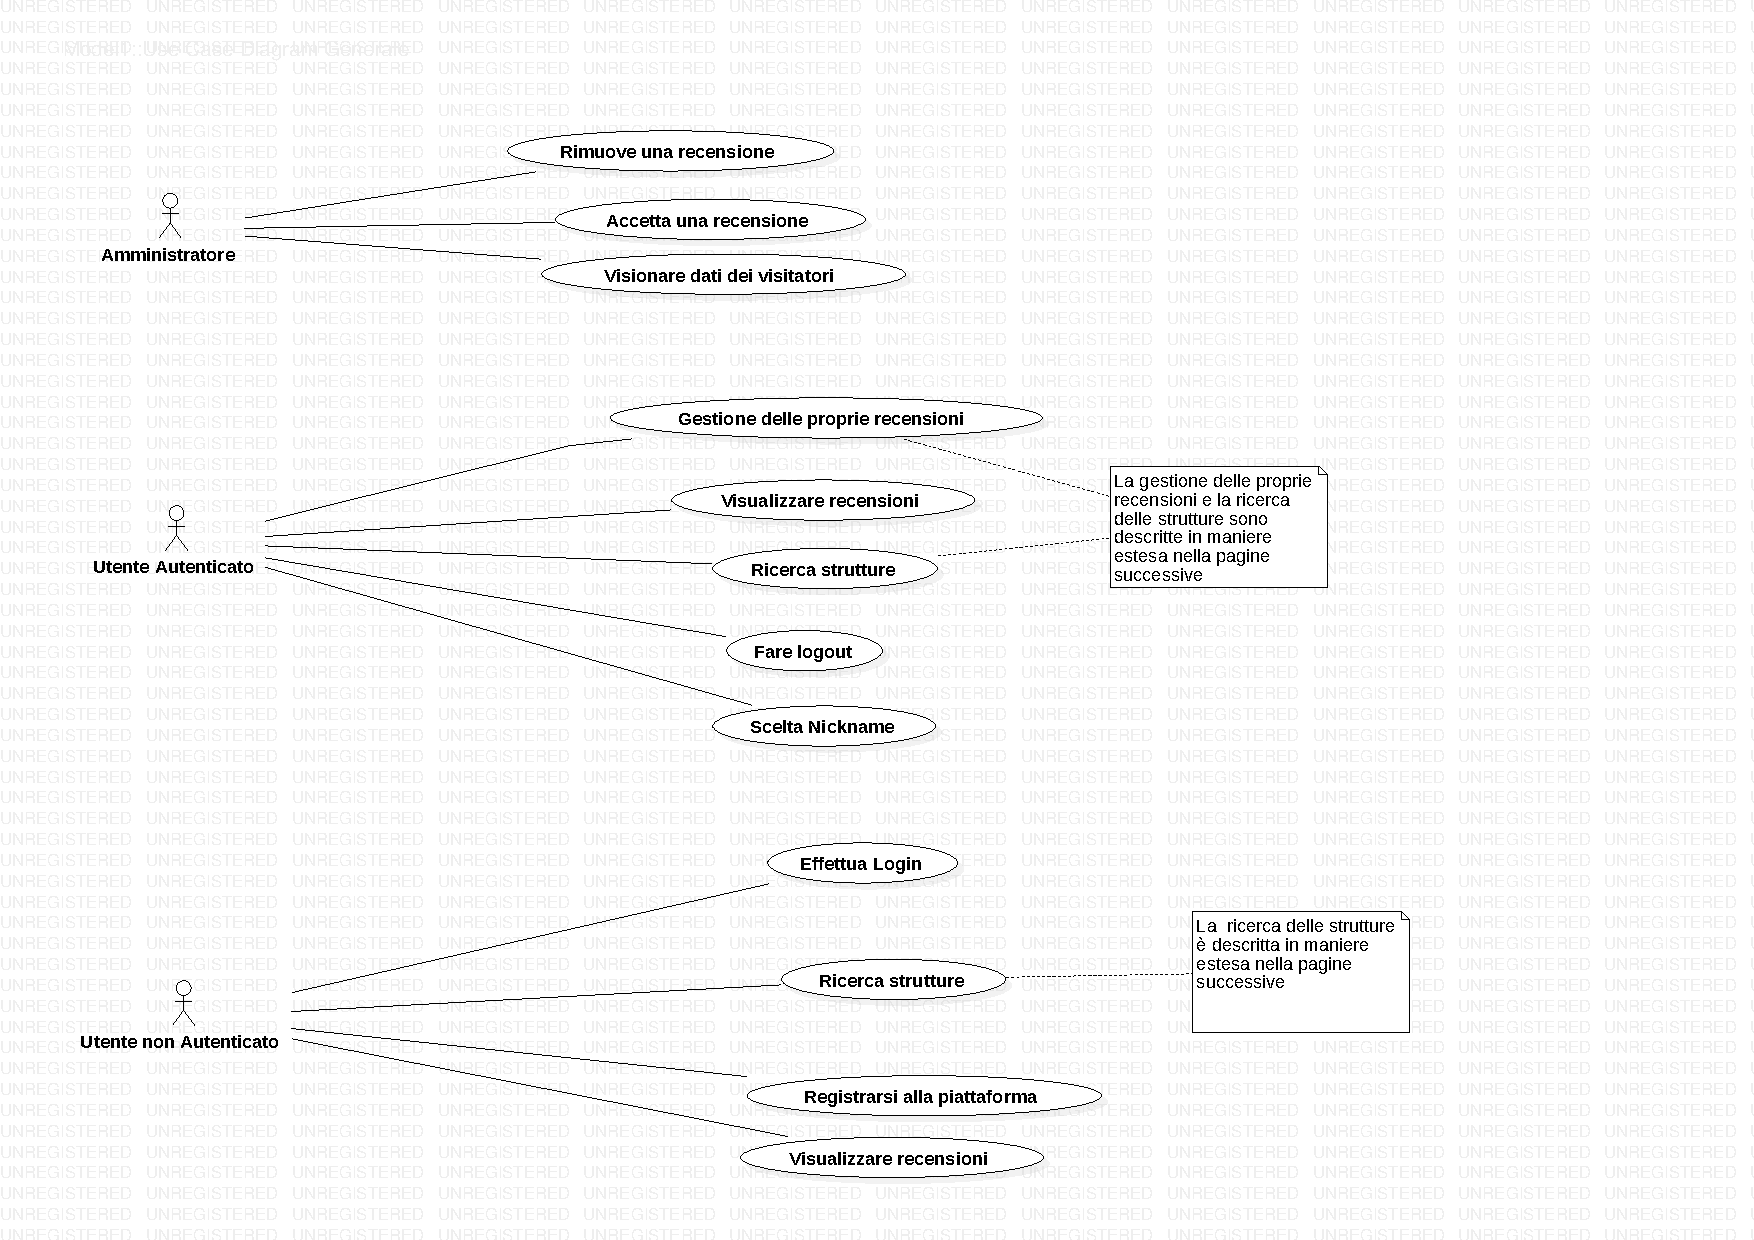
\includepdf[pages=-,nup={1x1}, angle=90]{usecase.pdf}
 
 \end{document}